\documentclass[aspectratio=169, 12pt]{beamer}

% --- Csomagok ---
\usepackage[utf8]{inputenc}
\usepackage[T1]{fontenc}
\usepackage[magyar]{babel}
\usepackage{graphicx}
\usepackage{booktabs}
\usepackage{tabularx}
\usepackage{hyperref}
\usepackage{multicol}
\usepackage{tikz}
\usetikzlibrary{arrows.meta, positioning, shapes.geometric, fit, calc}

% --- Tema ---
\usetheme{Madrid}
\usecolortheme{whale}

% Szinek testreszabasa
\definecolor{sapblue}{RGB}{0, 84, 150}
\definecolor{saplight}{RGB}{200, 220, 240}
\definecolor{sapgreen}{RGB}{50, 140, 80}
\definecolor{saporange}{RGB}{220, 120, 30}
\setbeamercolor{palette primary}{bg=sapblue, fg=white}
\setbeamercolor{palette secondary}{bg=sapblue!80, fg=white}
\setbeamercolor{palette tertiary}{bg=sapblue!60, fg=white}
\setbeamercolor{structure}{fg=sapblue}
\setbeamercolor{title}{fg=white, bg=sapblue}
\setbeamercolor{frametitle}{fg=white, bg=sapblue}
\setbeamercolor{block title}{bg=sapblue, fg=white}
\setbeamercolor{block body}{bg=saplight, fg=black}
\setbeamercolor{block title alerted}{bg=saporange, fg=white}
\setbeamercolor{block body alerted}{bg=saporange!10, fg=black}
\setbeamercolor{block title example}{bg=sapgreen, fg=white}
\setbeamercolor{block body example}{bg=sapgreen!10, fg=black}
\setbeamercolor{item}{fg=sapblue}

% Navigacio eltavolitasa
\setbeamertemplate{navigation symbols}{}
\setbeamertemplate{footline}{
  \leavevmode%
  \hbox{%
    \begin{beamercolorbox}[wd=.333333\paperwidth,ht=2.25ex,dp=1ex,center]{author in head/foot}%
      \usebeamerfont{author in head/foot}\insertshortauthor
    \end{beamercolorbox}%
    \begin{beamercolorbox}[wd=.333333\paperwidth,ht=2.25ex,dp=1ex,center]{title in head/foot}%
      \usebeamerfont{title in head/foot}\insertshorttitle
    \end{beamercolorbox}%
    \begin{beamercolorbox}[wd=.333333\paperwidth,ht=2.25ex,dp=1ex,right]{date in head/foot}%
      \usebeamerfont{date in head/foot}\insertshortdate{}\hspace*{2em}
      \insertframenumber{} / \inserttotalframenumber\hspace*{2ex}
    \end{beamercolorbox}}%
  \vskip0pt%
}

% --- Cimoldal informaciok ---
\title[Generatív AI]{Generatív AI és alkalmazások}
\author[Pál László]{Pál László}
\institute[Sapientia EMTE]{Sapientia EMTE, Csíkszereda}
\date{2026}

% ============================================================
\begin{document}

% ============================================================
%  I. RÉSZ — Bevezetés és történet
% ============================================================

% --- 1. dia: Cimlap ---
\begin{frame}[plain]
  \titlepage
\end{frame}

% --- 2. dia: A kobaltatol a generativ MI-ig ---
\begin{frame}{A kőbaltától a generatív MI-ig}
  \begin{columns}[T,onlytextwidth]
    \begin{column}{0.65\textwidth}
      \centering
      \begin{tabular}{cccc}
        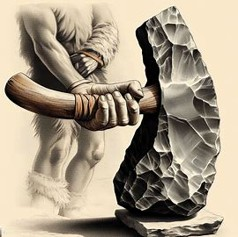
\includegraphics[width=2cm]{kepek/1_dia/Picture1.jpg} &
        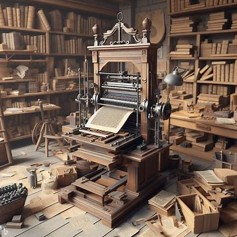
\includegraphics[width=2cm]{kepek/1_dia/Picture2.jpg} &
        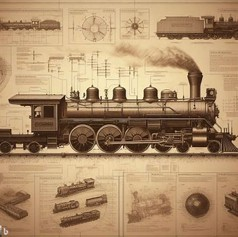
\includegraphics[width=2cm]{kepek/1_dia/Picture3.jpg} &
        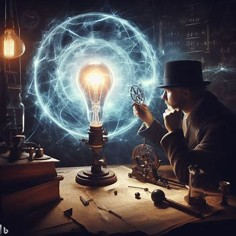
\includegraphics[width=2cm]{kepek/1_dia/Picture4.jpg} \\
        & {\scriptsize 15.\ század} & {\scriptsize 1879} & {\scriptsize 1878} \\[0.3cm]
        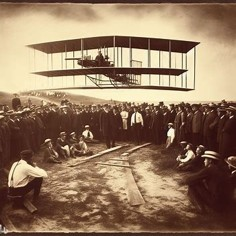
\includegraphics[width=2cm]{kepek/1_dia/Picture5.jpg} &
        
\includegraphics[width=2cm]{kepek/1_dia/Picture6.jpg} &
        
\includegraphics[width=2cm]{kepek/1_dia/Picture7.jpg} &
        
\includegraphics[width=2cm]{kepek/1_dia/Picture8.jpg} \\
        {\scriptsize 1903} & {\scriptsize 1920} & {\scriptsize 1935} & {\scriptsize 1990} \\
      \end{tabular}
    \end{column}
    \begin{column}{0.3\textwidth}
      \centering
      \vspace{1.5cm}
      
\includegraphics[width=2.5cm]{kepek/1_dia/Picture9.jpg} \\
      {\scriptsize 2022}
    \end{column}
  \end{columns}
\end{frame}

% --- 3. dia: MI kronologia ---
\begin{frame}{MI kronológia}
  \footnotesize
  \begin{columns}[T,onlytextwidth]
    \begin{column}{0.47\textwidth}
      \begin{itemize}\setlength{\itemsep}{1pt}
        \item \textbf{1950-es--60-as évek: a kezdetek}
          \begin{itemize}\setlength{\itemsep}{1pt}
            \item 1950: Turing teszt
            \item 1955: MI születése (Dartmouth)
            \item 1957: Perceptron
            \item 1958: Lisp nyelv
            \item 1965: ELIZA -- első chatbot
          \end{itemize}
        \item \textbf{1970--80-as évek: szakértői rendszerek}
          \begin{itemize}\setlength{\itemsep}{1pt}
            \item 1972: Dendral -- szakértői rendszer
            \item 1980-as évek: ,,AI Winter''
            \item 1986: Backpropagation
          \end{itemize}
      \end{itemize}
    \end{column}
    \begin{column}{0.47\textwidth}
      \begin{itemize}\setlength{\itemsep}{1pt}
        \item \textbf{1990--2000-es évek: gépi tanulás}
          \begin{itemize}\setlength{\itemsep}{1pt}
            \item NLP, Computer Vision (CNN)
            \item 1997: Deep Blue sikere
          \end{itemize}
        \item \textbf{2010-es évek: Deep Learning}
          \begin{itemize}\setlength{\itemsep}{1pt}
            \item 2012: AlexNet -- CNN áttörés
            \item 2017: Transformer architektúra
          \end{itemize}
        \item \textbf{2022+: Generatív AI kora}
          \begin{itemize}\setlength{\itemsep}{1pt}
            \item 2022: ChatGPT
            \item 2023: GPT-4, Claude, Gemini
            \item 2024: Claude 3.5, Llama 3, Sora
            \item 2025: DeepSeek R1, GPT-5
            \item 2026: Gemini 3.1, Claude 4
          \end{itemize}
      \end{itemize}
    \end{column}
  \end{columns}
\end{frame}

% --- 4. dia: MI modszerek kategoriai ---
\begin{frame}{MI módszerek kategóriái}
  \footnotesize
  \begin{columns}[T,onlytextwidth]
    \begin{column}{0.47\textwidth}
      \begin{block}{Felügyelt tanulás}
        Osztályozás, regresszió\\
        {\small\color{gray} Címkézett adatokból tanul}
      \end{block}
      \begin{block}{Felügyelet nélküli tanulás}
        Klaszterezés, dimenziócsökkentés\\
        {\small\color{gray} Rejtett mintákat keres}
      \end{block}
      \begin{block}{Megerősítéses tanulás}
        Játékok, robotika, optimalizálás\\
        {\small\color{gray} Jutalom alapján tanul}
      \end{block}
    \end{column}
    \begin{column}{0.47\textwidth}
      \begin{block}{Mélytanulás (Deep Learning)}
        CNN (képfelismerés)\\
        RNN / LSTM (szöveg, idősor)\\
        Transformer
      \end{block}
      \begin{alertblock}{Generatív AI}
        \textbf{Nagy nyelvi modellek (LLM)}\\
        Képgenerálás, hangszintézis, videó
      \end{alertblock}
    \end{column}
  \end{columns}
\end{frame}

% --- 5. dia: Neuronhalo abrak (TikZ) ---
\begin{frame}{A neurális hálók fejlődése}
  \begin{columns}[T,onlytextwidth]
    %--- Bal oszlop: Perceptron + MLP ---
    \begin{column}{0.48\textwidth}
      \centering
      % -- Perceptron --
      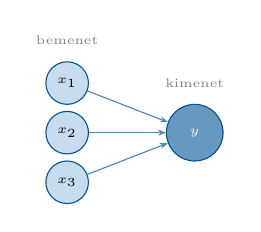
\begin{tikzpicture}[scale=0.9, every node/.style={scale=0.9},
        neur/.style={circle, draw=sapblue, fill=saplight, minimum size=6mm, inner sep=0pt, font=\tiny},
        outn/.style={circle, draw=sapblue, fill=sapblue!60, text=white, minimum size=8mm, inner sep=0pt, font=\tiny},
        conn/.style={-{Stealth[length=1mm]}, sapblue!70},
        lbl/.style={font=\tiny\color{gray}}
      ]
        \node[neur] (x1) at (0, 0.7) {$x_1$};
        \node[neur] (x2) at (0, 0)   {$x_2$};
        \node[neur] (x3) at (0,-0.7) {$x_3$};
        \node[outn] (y)  at (1.8, 0)  {$y$};
        \foreach \i in {1,2,3} { \draw[conn] (x\i) -- (y); }
        \node[lbl, above=1mm of x1] {bemenet};
        \node[lbl, above=1mm of y] {kimenet};
      \end{tikzpicture}\\[1pt]
      \textbf{Perceptron} {\small (1957)}

      \vspace{0.3cm}

      % -- MLP --
      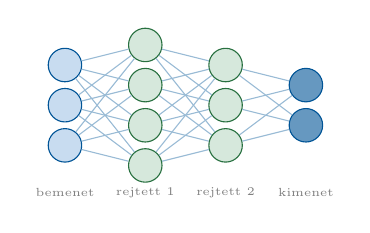
\begin{tikzpicture}[scale=0.85, every node/.style={scale=0.85},
        neur/.style={circle, draw=sapblue, fill=saplight, minimum size=5mm, inner sep=0pt},
        hidn/.style={circle, draw=sapgreen!80!black, fill=sapgreen!20, minimum size=5mm, inner sep=0pt},
        outn/.style={circle, draw=sapblue, fill=sapblue!60, minimum size=5mm, inner sep=0pt},
        conn/.style={sapblue!40},
        lbl/.style={font=\tiny\color{gray}}
      ]
        \foreach \i in {1,...,3} { \node[neur] (i\i) at (0, 1-\i*0.6) {}; }
        \foreach \j in {1,...,4} { \node[hidn] (h\j) at (1.2, 1.3-\j*0.6) {}; }
        \foreach \k in {1,...,3} { \node[hidn] (g\k) at (2.4, 1-\k*0.6) {}; }
        \foreach \o in {1,2} { \node[outn] (o\o) at (3.6, 0.7-\o*0.6) {}; }
        \foreach \i in {1,...,3} \foreach \j in {1,...,4} { \draw[conn] (i\i) -- (h\j); }
        \foreach \j in {1,...,4} \foreach \k in {1,...,3} { \draw[conn] (h\j) -- (g\k); }
        \foreach \k in {1,...,3} \foreach \o in {1,2} { \draw[conn] (g\k) -- (o\o); }
        \node[lbl] at (0, -1.5) {bemenet};
        \node[lbl] at (1.2, -1.5) {rejtett 1};
        \node[lbl] at (2.4, -1.5) {rejtett 2};
        \node[lbl] at (3.6, -1.5) {kimenet};
      \end{tikzpicture}\\[1pt]
      \textbf{Többrétegű perceptron} (MLP)\\
      {\scriptsize\color{gray} Több réteg → nemlineáris problémák}
    \end{column}
    %--- Jobb oszlop: Backprop + Deep NN ---
    \begin{column}{0.48\textwidth}
      \centering
      % -- Backpropagation --
      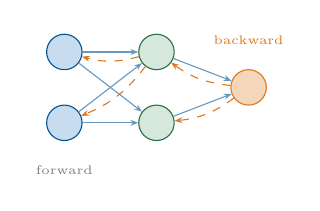
\begin{tikzpicture}[scale=0.9, every node/.style={scale=0.9},
        neur/.style={circle, draw=sapblue, fill=saplight, minimum size=5mm, inner sep=0pt},
        hidn/.style={circle, draw=sapgreen!80!black, fill=sapgreen!20, minimum size=5mm, inner sep=0pt},
        outn/.style={circle, draw=saporange, fill=saporange!30, minimum size=5mm, inner sep=0pt},
        fwd/.style={-{Stealth[length=1mm]}, sapblue!60},
        bwd/.style={-{Stealth[length=1mm]}, saporange, dashed},
        lbl/.style={font=\tiny\color{gray}}
      ]
        \node[neur] (i1) at (0, 0.5)  {};
        \node[neur] (i2) at (0,-0.5) {};
        \node[hidn] (h1) at (1.3, 0.5)  {};
        \node[hidn] (h2) at (1.3,-0.5) {};
        \node[outn] (o1) at (2.6, 0) {};
        \foreach \i in {1,2} \foreach \j in {1,2} { \draw[fwd] (i\i) -- (h\j); }
        \foreach \j in {1,2} { \draw[fwd] (h\j) -- (o1); }
        \foreach \j in {1,2} { \draw[bwd] (o1) to[bend left=15] (h\j); }
        \foreach \i in {1,2} { \draw[bwd] (h1) to[bend left=15] (i\i); }
        \node[lbl, below=2mm of i2] {forward};
        \node[lbl, above=2mm of o1, text=saporange] {backward};
      \end{tikzpicture}\\[1pt]
      \textbf{Backpropagation} {\small (1986)}\\
      {\scriptsize\color{gray} Hiba visszaterjesztése a súlyok frissítéséhez}

      \vspace{0.3cm}

      % -- Deep Neural Network --
      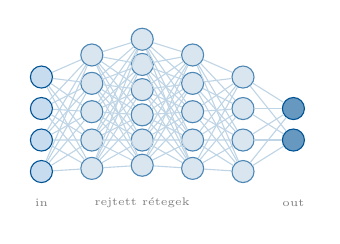
\begin{tikzpicture}[scale=0.8, every node/.style={scale=0.8},
        neur/.style={circle, draw=sapblue, fill=saplight, minimum size=3.5mm, inner sep=0pt},
        hidn/.style={circle, draw=sapblue!70, fill=sapblue!15, minimum size=3.5mm, inner sep=0pt},
        outn/.style={circle, draw=sapblue, fill=sapblue!60, minimum size=3.5mm, inner sep=0pt},
        conn/.style={sapblue!25},
        lbl/.style={font=\tiny\color{gray}}
      ]
        \foreach \i in {1,...,4} { \node[neur] (i\i) at (0, 1-\i*0.5) {}; }
        \foreach \j in {1,...,5} { \node[hidn] (a\j) at (0.8, 1.3-\j*0.45) {}; }
        \foreach \k in {1,...,6} { \node[hidn] (b\k) at (1.6, 1.5-\k*0.4) {}; }
        \foreach \l in {1,...,5} { \node[hidn] (c\l) at (2.4, 1.3-\l*0.45) {}; }
        \foreach \m in {1,...,4} { \node[hidn] (d\m) at (3.2, 1-\m*0.5) {}; }
        \foreach \o in {1,2} { \node[outn] (o\o) at (4.0, 0.5-\o*0.5) {}; }
        \foreach \i in {1,...,4} \foreach \j in {1,...,5} { \draw[conn] (i\i) -- (a\j); }
        \foreach \j in {1,...,5} \foreach \k in {1,...,6} { \draw[conn] (a\j) -- (b\k); }
        \foreach \k in {1,...,6} \foreach \l in {1,...,5} { \draw[conn] (b\k) -- (c\l); }
        \foreach \l in {1,...,5} \foreach \m in {1,...,4} { \draw[conn] (c\l) -- (d\m); }
        \foreach \m in {1,...,4} \foreach \o in {1,2} { \draw[conn] (d\m) -- (o\o); }
        \node[lbl] at (0, -1.5) {in};
        \node[lbl] at (1.6, -1.5) {rejtett rétegek};
        \node[lbl] at (4.0, -1.5) {out};
      \end{tikzpicture}\\[1pt]
      \textbf{Mély neurális háló} (DNN)
    \end{column}
  \end{columns}
\end{frame}

% ============================================================
%  II. RÉSZ — Nagy nyelvi modellek
% ============================================================

% --- 6. dia: LLM bevezeto ---
\begin{frame}{Nagy nyelvi modellek (LLM)}
  \footnotesize
  \begin{itemize}\setlength{\itemsep}{1pt}
    \item \textbf{LLM}: transformer alapú neurális háló, amely a \textbf{következő token valószínűségét} tanulja
    \item \textbf{Transformer architektúra} -- a modern LLM-ek alapja (2017, Google: ,,\textit{Attention is All You Need}'')
    \item Hatalmas szövegkorpuszon tanítják (internet, könyvek, kód) -- milliárdos paraméterszám
  \end{itemize}

  \vspace{0.2cm}
  \centering
  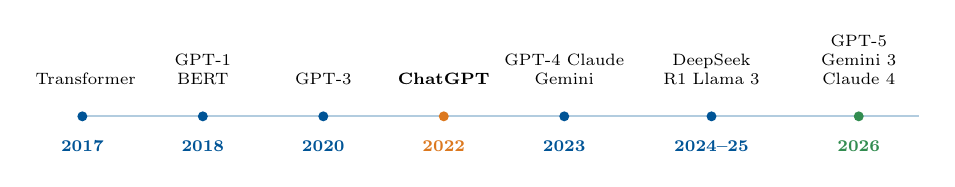
\begin{tikzpicture}[scale=0.85, every node/.style={scale=0.85},
    dot/.style={circle, fill=sapblue, inner sep=1.5pt},
    yr/.style={font=\scriptsize\bfseries, text=sapblue},
    ev/.style={font=\scriptsize, text width=1.4cm, align=center},
    evw/.style={font=\scriptsize, text width=1.8cm, align=center}
  ]
    \draw[thick, sapblue!30] (0,0) -- (12.5,0);
    % 2017
    \node[dot] (d1) at (0,0) {};
    \node[yr, below=2mm] at (d1) {2017};
    \node[ev, above=3mm] at (d1) {Transformer};
    % 2018
    \node[dot] (d2) at (1.8,0) {};
    \node[yr, below=2mm] at (d2) {2018};
    \node[ev, above=3mm] at (d2) {GPT-1 BERT};
    % 2020
    \node[dot] (d3) at (3.6,0) {};
    \node[yr, below=2mm] at (d3) {2020};
    \node[ev, above=3mm] at (d3) {GPT-3};
    % 2022
    \node[dot, fill=saporange] (d4) at (5.4,0) {};
    \node[yr, below=2mm, text=saporange] at (d4) {2022};
    \node[ev, above=3mm] at (d4) {\textbf{ChatGPT}};
    % 2023
    \node[dot] (d5) at (7.2,0) {};
    \node[yr, below=2mm] at (d5) {2023};
    \node[evw, above=3mm] at (d5) {GPT-4 Claude Gemini};
    % 2024–25
    \node[dot] (d6) at (9.4,0) {};
    \node[yr, below=2mm] at (d6) {2024--25};
    \node[evw, above=3mm] at (d6) {DeepSeek R1 Llama 3};
    % 2026
    \node[dot, fill=sapgreen] (d7) at (11.6,0) {};
    \node[yr, below=2mm, text=sapgreen] at (d7) {2026};
    \node[evw, above=3mm] at (d7) {GPT-5 Gemini 3 Claude 4};
  \end{tikzpicture}
\end{frame}

% --- 7. dia: LLM lehetosegek, kihivasok ---
\begin{frame}{LLM -- Lehetőségek és kihívások}
  \footnotesize
  \begin{columns}[T,onlytextwidth]
    \begin{column}{0.47\textwidth}
      \begin{exampleblock}{Lehetőségek}
        \begin{itemize}\setlength{\itemsep}{1pt}
          \item Szöveggenerálás
          \item Fordítás
          \item Összefoglalás
          \item Kódelőállítás
          \item Osztályozás, kategorizálás
          \item Sentiment elemzés
          \item Chatbotok, asszisztensek
        \end{itemize}
      \end{exampleblock}
    \end{column}
    \begin{column}{0.47\textwidth}
      \begin{alertblock}{Kihívások}
        \begin{itemize}\setlength{\itemsep}{1pt}
          \item Költséges (erőforrás-igény)
          \item \textbf{Hallucinálás}
          \item Megbízhatóság, pontosság
          \item Adatvédelem, etika
        \end{itemize}
      \end{alertblock}
      \begin{block}{Alkalmazások}
        \begin{itemize}\setlength{\itemsep}{1pt}
          \item Egészségügy, pénzügy
          \item Marketing, oktatás
          \item Szoftverfejlesztés
        \end{itemize}
      \end{block}
    \end{column}
  \end{columns}
\end{frame}

% --- 8. dia: Hogyan mukodik? ---
% KÉP SZÜKSÉGES: kepek/8_dia/ mappába: llm_pipeline.png, token_probs.png
\begin{frame}{Hogyan működik egy LLM?}
  \footnotesize
  \begin{columns}[T,onlytextwidth]
    \begin{column}{0.52\textwidth}
      \centering
      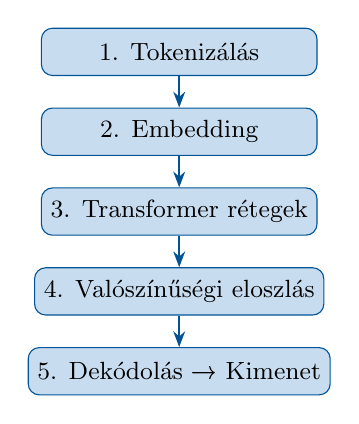
\begin{tikzpicture}[
        node distance=0.4cm,
        box/.style={draw=sapblue, fill=saplight, rounded corners, minimum width=3.5cm, minimum height=0.6cm, font=\small, align=center},
        arr/.style={-{Stealth[length=2mm]}, thick, sapblue}
      ]
        \node[box] (tok) {1. Tokenizálás};
        \node[box, below=of tok] (emb) {2. Embedding};
        \node[box, below=of emb] (mod) {3. Transformer rétegek};
        \node[box, below=of mod] (prob) {4. Valószínűségi eloszlás};
        \node[box, below=of prob] (dec) {5. Dekódolás → Kimenet};
        \draw[arr] (tok) -- (emb);
        \draw[arr] (emb) -- (mod);
        \draw[arr] (mod) -- (prob);
        \draw[arr] (prob) -- (dec);
      \end{tikzpicture}
    \end{column}
    \begin{column}{0.42\textwidth}
      \begin{block}{Következő szó predikció}
        ,,The cat sat on the \textbf{...}''

        \vspace{0.2cm}

        {\small
        \begin{tabular}{lr}
          mat & 45\% \\
          floor & 22\% \\
          table & 15\% \\
          roof & 8\% \\
          ... & ... \\
        \end{tabular}}
      \end{block}

      \vspace{0.3cm}
      {\small A modell mindig a legvalószínűbb következő tokent választja (vagy mintavételez).}
    \end{column}
  \end{columns}
\end{frame}

% --- 9. dia: Token, kontextus, temperature, hallucinacio ---
\begin{frame}{Alapfogalmak}
  \footnotesize
  \begin{columns}[T,onlytextwidth]
    \begin{column}{0.47\textwidth}
      \begin{block}{Token}
        \begin{itemize}\setlength{\itemsep}{1pt}
          \item A szöveg legkisebb egysége
          \item 1 token $\approx$ 0,75 szó (kb.\ 4 karakter)
          \item A modell tokeneket olvas, nem szavakat
        \end{itemize}
      \end{block}
      \begin{block}{Kontextus ablak}
        \begin{itemize}\setlength{\itemsep}{1pt}
          \item Amit a modell egyszerre ,,lát''
          \item GPT-3: 4k → Gemini 3: \textbf{1\,000\,000} token
          \item 1M token $\approx$ \textbf{10 könyv} (750k szó)
          \item Nem fér bele → ,,elfelejti''
        \end{itemize}
      \end{block}
    \end{column}
    \begin{column}{0.47\textwidth}
      \begin{block}{Temperature}
        \begin{itemize}\setlength{\itemsep}{1pt}
          \item Generálás véletlenszerűsége
          \item 0 = determinisztikus (kódoláshoz)
          \item 1 = kreatív (ötleteléshez)
        \end{itemize}
      \end{block}
      \begin{alertblock}{Hallucinálás}
        \begin{itemize}\setlength{\itemsep}{1pt}
          \item Magabiztosan állít valótlant
          \item Nem hazugság: statisztikailag valószínű szöveget generál
          \item \textbf{Mindig ellenőrizz!}
        \end{itemize}
      \end{alertblock}
    \end{column}
  \end{columns}
\end{frame}

% --- 10. dia: RAG ---
\begin{frame}{RAG -- Retrieval-Augmented Generation}
  \footnotesize
  \begin{columns}[T,onlytextwidth]
    \begin{column}{0.52\textwidth}
      \centering
      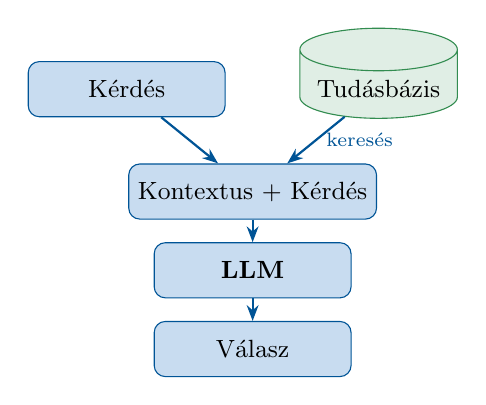
\begin{tikzpicture}[
        node distance=0.5cm,
        box/.style={draw=sapblue, fill=saplight, rounded corners, minimum width=2.5cm, minimum height=0.7cm, font=\small, align=center},
        db/.style={draw=sapgreen, fill=sapgreen!15, cylinder, shape border rotate=90, aspect=0.3, minimum width=2cm, minimum height=0.8cm, font=\small},
        arr/.style={-{Stealth[length=2mm]}, thick, sapblue}
      ]
        \node[box] (query) at (0,0) {Kérdés};
        \node[db]  (db)    at (3.2,0) {Tudásbázis};
        \node[box] (ctx)   at (1.6,-1.3) {Kontextus + Kérdés};
        \node[box] (llm)   at (1.6,-2.3) {\textbf{LLM}};
        \node[box] (ans)   at (1.6,-3.3) {Válasz};
        \draw[arr] (query) -- (ctx);
        \draw[arr] (db) -- node[right, font=\scriptsize]{keresés} (ctx);
        \draw[arr] (ctx) -- (llm);
        \draw[arr] (llm) -- (ans);
      \end{tikzpicture}
    \end{column}
    \begin{column}{0.42\textwidth}
      \begin{block}{Mi ez?}
        A modell saját dokumentumokból keres releváns részleteket, és azok alapján válaszol.
      \end{block}

      \vspace{0.3cm}

      \begin{exampleblock}{Miért fontos?}
        \begin{itemize}\setlength{\itemsep}{1pt}
          \item Csökkenti a hallucinálást
          \item Naprakész tudás
          \item Nem kell újratanítani
        \end{itemize}
      \end{exampleblock}

    \end{column}
  \end{columns}
\end{frame}

% --- 11. dia: Fine-tuning ---
\begin{frame}{Fine-tuning -- Finomhangolás}
  \footnotesize
  \begin{columns}[T,onlytextwidth]
    \begin{column}{0.47\textwidth}
      \begin{block}{Mi ez?}
        Egy előtanított modell \textbf{további tanítása} saját adatokon, hogy jobban illeszkedjen egy konkrét feladathoz.
      \end{block}

      \vspace{0.3cm}

      \begin{exampleblock}{Mikor érdemes?}
        \begin{itemize}\setlength{\itemsep}{1pt}
          \item Speciális szakterület (orvosi, jogi)
          \item Egyedi stílus vagy formátum
          \item Nagy mennyiségű saját adat
        \end{itemize}
      \end{exampleblock}
    \end{column}
    \begin{column}{0.47\textwidth}
      \begin{alertblock}{RAG vs Fine-tuning}
        \begin{tabular}{lcc}
          & \textbf{RAG} & \textbf{Fine-tune} \\
          \midrule
          Költség & Alacsony & Magas \\
          Frissesség & Azonnali & Újratanítás \\
          Pontosság & Jó & Nagyon jó \\
          Beállítás & Egyszerű & Összetett \\
        \end{tabular}
      \end{alertblock}

      \vspace{0.3cm}

      {\small A gyakorlatban a \textbf{RAG} az elterjedtebb megoldás -- gyorsabb, olcsóbb, rugalmasabb.}
    \end{column}
  \end{columns}
\end{frame}

% ============================================================
%  III. RÉSZ — Új trendek és technológiák
% ============================================================

% --- 12. dia: Multimodalitas ---
\begin{frame}{Multimodalitás}
  \footnotesize
  \begin{columns}[T,onlytextwidth]
    \begin{column}{0.43\textwidth}
      \begin{block}{Mi ez?}
        Egyetlen modell \textbf{többféle} bemenetet és kimenetet kezel:
      \end{block}

      \vspace{0.2cm}

      \centering
      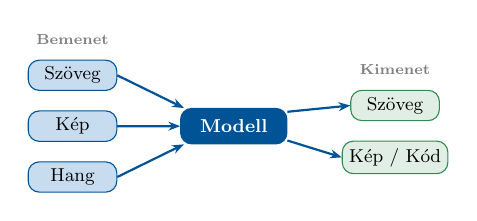
\begin{tikzpicture}[scale=0.75, every node/.style={scale=0.75},
        node distance=0.25cm,
        inp/.style={draw=sapblue, fill=saplight, rounded corners, minimum width=1.5cm, minimum height=0.45cm, font=\small},
        llm/.style={draw=sapblue, fill=sapblue, text=white, rounded corners, minimum width=1.8cm, minimum height=0.6cm, font=\small\bfseries},
        outp/.style={draw=sapgreen, fill=sapgreen!15, rounded corners, minimum width=1.5cm, minimum height=0.45cm, font=\small},
        arr/.style={-{Stealth[length=1.5mm]}, thick, sapblue},
        grp/.style={font=\scriptsize\bfseries, text=gray}
      ]
        \node[inp] (t) {Szöveg};
        \node[inp, below=of t] (i) {Kép};
        \node[inp, below=of i] (a) {Hang};
        \node[llm, right=0.8cm of i] (m) {Modell};
        \node[outp, right=0.8cm of m, yshift=0.35cm] (o1) {Szöveg};
        \node[outp, below=of o1] (o2) {Kép / Kód};
        \draw[arr] (t.east) -- (m.160);
        \draw[arr] (i.east) -- (m.west);
        \draw[arr] (a.east) -- (m.200);
        \draw[arr] (m.15) -- (o1.west);
        \draw[arr] (m.345) -- (o2.west);
        % Bemenet / Kimenet feliratok
        \node[grp, above=1mm of t] {Bemenet};
        \node[grp, above=1mm of o1] {Kimenet};
      \end{tikzpicture}
    \end{column}
    \begin{column}{0.47\textwidth}
      \begin{exampleblock}{Multimodális modellek}
        \begin{itemize}\setlength{\itemsep}{1pt}
          \item \textbf{GPT-5 / o3} -- szöveg, kép, hang
          \item \textbf{Gemini 3} -- szöveg, kép, hang, videó
          \item \textbf{Claude 4} -- szöveg, kép, kód
        \end{itemize}
      \end{exampleblock}

      \vspace{0.3cm}

      \begin{block}{Példák a gyakorlatban}
        \begin{itemize}\setlength{\itemsep}{1pt}
          \item Kép leírása szöveggel
          \item PDF dokumentum feldolgozás
          \item Hangfelvétel elemzése
          \item Videó összefoglalás
        \end{itemize}
      \end{block}
    \end{column}
  \end{columns}
\end{frame}

% --- 13. dia: AI agensek ---
\begin{frame}{AI ágensek}
  \footnotesize
  \begin{columns}[T,onlytextwidth]
    \begin{column}{0.47\textwidth}
      \begin{block}{Mi az ágens?}
        Olyan AI rendszer, amely \textbf{önállóan tervez és cselekszik}: eszközöket használ, döntéseket hoz, és iteratívan oldja meg a feladatot.
      \end{block}

      \vspace{0.2cm}

      \centering
      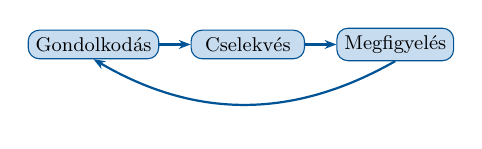
\begin{tikzpicture}[scale=0.8, every node/.style={scale=0.8},
        node distance=0.4cm,
        box/.style={draw=sapblue, fill=saplight, rounded corners, minimum width=1.8cm, minimum height=0.45cm, font=\small, align=center},
        arr/.style={-{Stealth[length=1.5mm]}, thick, sapblue}
      ]
        \node[box] (think) {Gondolkodás};
        \node[box, right=of think] (act) {Cselekvés};
        \node[box, right=of act] (obs) {Megfigyelés};
        \draw[arr] (think) -- (act);
        \draw[arr] (act) -- (obs);
        \draw[arr, bend left=30] (obs.south) to (think.south);
      \end{tikzpicture}
    \end{column}
    \begin{column}{0.47\textwidth}
      \begin{exampleblock}{Képességek}
        \begin{itemize}\setlength{\itemsep}{1pt}
          \item Webkeresés, fájlkezelés
          \item Kódfuttatás
          \item API-k hívása (,,tool use'')
          \item Többlépéses feladatok
        \end{itemize}
      \end{exampleblock}

      \vspace{0.1cm}

      \begin{block}{Példák}
        \begin{itemize}\setlength{\itemsep}{1pt}
          \item \textbf{Claude Code} -- programozó ágens
          \item \textbf{Devin} -- szoftverfejlesztő ágens
          \item \textbf{Manus} -- általános célú ágens
          \item \textbf{OpenAI Operator} -- böngésző ágens
        \end{itemize}
      \end{block}
    \end{column}
  \end{columns}
\end{frame}

% --- 14. dia: MCP protokoll ---
\begin{frame}{MCP -- Model Context Protocol}
  \footnotesize
  \begin{columns}[T,onlytextwidth]
    \begin{column}{0.47\textwidth}
      \begin{block}{Mi ez?}
        \textbf{Nyílt szabvány} (Anthropic, 2024), amely egységes módon kapcsolja össze az LLM-eket külső eszközökkel és adatforrásokkal.
      \end{block}

      \vspace{0.3cm}

      \centering
      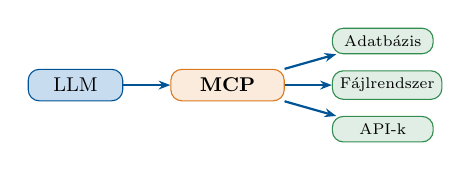
\begin{tikzpicture}[scale=0.8, every node/.style={scale=0.8},
        node distance=0.4cm,
        box/.style={draw=sapblue, fill=saplight, rounded corners, minimum width=1.5cm, minimum height=0.5cm, font=\small, align=center},
        mcp/.style={draw=saporange, fill=saporange!15, rounded corners, minimum width=1.8cm, minimum height=0.5cm, font=\small\bfseries, align=center},
        tool/.style={draw=sapgreen, fill=sapgreen!15, rounded corners, minimum width=1.6cm, minimum height=0.4cm, font=\scriptsize, align=center},
        arr/.style={-{Stealth[length=1.5mm]}, thick, sapblue}
      ]
        \node[box] (llm) {LLM};
        \node[mcp, right=0.6cm of llm] (mcp) {MCP};
        \node[tool, right=0.6cm of mcp, yshift=0.7cm] (t1) {Adatbázis};
        \node[tool, right=0.6cm of mcp] (t2) {Fájlrendszer};
        \node[tool, right=0.6cm of mcp, yshift=-0.7cm] (t3) {API-k};
        \draw[arr] (llm) -- (mcp);
        \draw[arr] (mcp) -- (t1);
        \draw[arr] (mcp) -- (t2);
        \draw[arr] (mcp) -- (t3);
      \end{tikzpicture}
    \end{column}
    \begin{column}{0.43\textwidth}
      \begin{exampleblock}{Miért fontos?}
        \begin{itemize}\setlength{\itemsep}{1pt}
          \item Egy szabvány, sok eszköz
          \item Bármely LLM használhatja
          \item Kliens--szerver architektúra
          \item Növekvő ökoszisztéma
        \end{itemize}
      \end{exampleblock}

      \vspace{0.3cm}

      {\small Analógia: ahogy az \textbf{USB} szabványosította a hardver csatlakoztatást, az \textbf{MCP} szabványosítja az AI eszközökhöz való hozzáférést.}
    \end{column}
  \end{columns}
\end{frame}

% --- 15. dia: Vibe coding ---
\begin{frame}{Vibe coding -- AI-asszisztált programozás}
  \footnotesize
  \begin{columns}[T,onlytextwidth]
    \begin{column}{0.47\textwidth}
      \begin{block}{Mi ez?}
        Természetes nyelven leírjuk, \textbf{mit} szeretnénk, és az AI megírja a kódot. A hangsúly az eredményen van, nem a szintaxison.
      \end{block}

      \vspace{0.3cm}

      \begin{alertblock}{Fontos}
        \begin{itemize}\setlength{\itemsep}{1pt}
          \item Nem váltja ki a programozási tudást
          \item Megérteni és ellenőrizni kell a kódot
          \item Nagyon hatékony prototipizáláshoz
        \end{itemize}
      \end{alertblock}
    \end{column}
    \begin{column}{0.47\textwidth}
      \begin{exampleblock}{Eszközök}
        \begin{itemize}\setlength{\itemsep}{1pt}
          \item \textbf{GitHub Copilot} -- kódkiegészítés IDE-ben
          \item \textbf{Cursor} -- AI-native szerkesztő
          \item \textbf{Claude Code} -- terminál alapú ágens
          \item \textbf{Windsurf} -- AI IDE
          \item \textbf{Gemini Code Assist}
        \end{itemize}
      \end{exampleblock}

      \vspace{0.2cm}

      {\small A kifejezést \textbf{Andrej Karpathy} használta először, 2025 februárjában.}
    \end{column}
  \end{columns}
\end{frame}

% ============================================================
%  IV. RÉSZ — Modellek világa 2026-ban
% ============================================================

% --- 16. dia: Fontosabb modellek ---
\begin{frame}{A modellek világa 2026-ban}
  \vspace{0.2cm}
  {\small
  \renewcommand{\arraystretch}{1.15}
  \begin{tabularx}{\textwidth}{l X l}
    \textbf{Modell} & \textbf{Jellemzők} & \textbf{Fejlesztő} \\
    \midrule
    GPT-5 / o3 & Legnépszerűbb, multimodális, reasoning & OpenAI \\
    Claude 4 (Opus/Sonnet) & Hosszú kontextus, precíz, kód, ágensek & Anthropic \\
    Gemini 3 & 1M kontextus, multimodális, ,,gondolkodó'' & Google \\
    Grok 4 & Valós idejű X adatok, reasoning & xAI \\
    Llama 4 & Nyílt forráskódú, lokálisan futtatható & Meta \\
    DeepSeek R1/V3 & Erős kód/matek, nyílt, költséghatékony & DeepSeek \\
    Mistral Large & Európai, hatékony, többnyelvű, nyílt & Mistral AI \\
  \end{tabularx}
  }
\end{frame}

% --- 17. dia: Modellek funkciok szerint ---
\begin{frame}{Modellek funkciók szerint}
  \begin{columns}[T,onlytextwidth]
    \begin{column}{0.47\textwidth}
      \begin{block}{Szöveg / Chat}
        \smallskip\footnotesize ChatGPT, Claude, Gemini, Grok, DeepSeek
      \end{block}
      \begin{block}{Programozás}
        \smallskip\footnotesize Claude Code, GitHub Copilot, Cursor, Gemini Code Assist, Windsurf, Antigravity
      \end{block}
      \begin{block}{Képgenerálás}
        \smallskip\footnotesize DALL·E 3, Midjourney, Stable Diffusion, Flux, Ideogram
      \end{block}
    \end{column}
    \begin{column}{0.47\textwidth}
      \begin{block}{Hang / Beszéd}
        \smallskip\footnotesize OpenAI Whisper (STT), ElevenLabs (TTS), NotebookLM
      \end{block}
      \begin{block}{Videó}
        \smallskip\footnotesize Sora (OpenAI), Runway, Kling, Veo 2 (Google)
      \end{block}
      \begin{block}{Zene}
        \smallskip\footnotesize Suno, Udio
      \end{block}
    \end{column}
  \end{columns}

  \vspace{0.3cm}
  \centering
  {\footnotesize\color{gray} A piac rendkívül gyorsan változik -- heti szinten jelennek meg új modellek és funkciók.}
\end{frame}

% --- 18. dia: Lokalis modellek es Hugging Face ---
\begin{frame}{Lokális modellek és Hugging Face}
  \footnotesize
  \begin{columns}[T,onlytextwidth]
    \begin{column}{0.47\textwidth}
      \begin{block}{Miért lokális modell?}
        \begin{itemize}\setlength{\itemsep}{1pt}
          \item Adatvédelem (adat nem hagyja el a gépet)
          \item Nincs előfizetési díj
          \item Offline működés
          \item Testreszabhatóság
        \end{itemize}
      \end{block}

      \vspace{0.2cm}

      \begin{exampleblock}{Futtatókörnyezetek}
        \begin{itemize}\setlength{\itemsep}{1pt}
          \item \textbf{Ollama} -- egyszerű CLI
          \item \textbf{LM Studio} -- grafikus felület
          \item \textbf{llama.cpp} -- optimalizált futtatás
        \end{itemize}
      \end{exampleblock}
    \end{column}
    \begin{column}{0.47\textwidth}
      \begin{block}{Hugging Face}
        \begin{itemize}\setlength{\itemsep}{1pt}
          \item Az AI közösség ,,GitHubja''
          \item Modellek, adatkészletek, demók
          \item 1\,000\,000+ modell elérhető
        \end{itemize}
      \end{block}

      \vspace{0.2cm}

      \begin{block}{Népszerű nyílt modellek}
        \begin{itemize}\setlength{\itemsep}{1pt}
          \item \textbf{Llama 4} (Meta) -- Scout, Maverick
          \item \textbf{Mistral Large} -- többnyelvű
          \item \textbf{Phi-4} (Microsoft) -- kisméretű
          \item \textbf{Gemma 3} (Google) -- nyílt
          \item \textbf{DeepSeek R1/V3} -- kód/matek
        \end{itemize}
      \end{block}
    \end{column}
  \end{columns}
\end{frame}

% ============================================================
%  V. RÉSZ — Prompt engineering és eszközök
% ============================================================

% --- 19. dia: Prompt engineering attekintes ---
\begin{frame}{Prompt engineering}
  \footnotesize
  \begin{columns}[T,onlytextwidth]
    \begin{column}{0.47\textwidth}
      \begin{block}{Prompt}
        Az utasítás vagy kérdés, amit a nyelvi modellnek adunk, hogy a \textbf{legjobb választ} kapjuk.
      \end{block}

      \vspace{0.3cm}

      \begin{block}{Prompt engineering}
        Hogyan fogalmazzuk meg az utasítást a \textbf{leghatékonyabban}:
        \begin{itemize}\setlength{\itemsep}{1pt}
          \item Megfelelő kontextus
          \item Egyértelmű elvárások
          \item Struktúra és formátum
        \end{itemize}
      \end{block}
    \end{column}
    \begin{column}{0.47\textwidth}
      \begin{exampleblock}{Technikák}
        \begin{itemize}\setlength{\itemsep}{1pt}
          \item \textbf{Zero-shot} -- utasítás példa nélkül
          \item \textbf{Few-shot} -- néhány példával
          \item \textbf{Chain of Thought} -- lépésről lépésre
          \item \textbf{Persona} -- szerep megadása
          \item \textbf{Negatív utasítás} -- mit ne tegyen
          \item \textbf{Reflexion} -- önellenőrzés
        \end{itemize}
      \end{exampleblock}

      \vspace{0.2cm}

      {\small Részletek az \textbf{1.\ feladatban} (Promptolás).}
    \end{column}
  \end{columns}
\end{frame}

% --- 20. dia: Gemini bemutato ---
\begin{frame}{Google Gemini}
  \footnotesize
  \begin{columns}[T,onlytextwidth]
    \begin{column}{0.52\textwidth}
      \begin{block}{Mi ez?}
        A Google multimodális AI modellje és chatfelülete.
        \begin{itemize}\setlength{\itemsep}{1pt}
          \item Ingyenesen elérhető
          \item Google fiókkal használható
          \item Szöveg, kép, dokumentum, kód
        \end{itemize}
      \end{block}

      \vspace{0.15cm}

      \begin{exampleblock}{Képességek}
        \begin{itemize}\setlength{\itemsep}{1pt}
          \item PDF feldolgozás
          \item Kép elemzése
          \item Kódgenerálás
          \item Google szolgáltatások integrációja
        \end{itemize}
      \end{exampleblock}
    \end{column}
    \begin{column}{0.42\textwidth}
      \vspace{1cm}
      \centering
      \url{https://gemini.google.com}

      \vspace{0.5cm}

      Használat: jelentkezzetek be a \textbf{saját email} címetekkel.
    \end{column}
  \end{columns}
\end{frame}

% --- 21. dia: Google Colab bemutato ---
\begin{frame}{Google Colab}
  \footnotesize
  \begin{columns}[T,onlytextwidth]
    \begin{column}{0.52\textwidth}
      \begin{block}{Mi ez?}
        Felhőalapú \textbf{Python notebook} környezet, közvetlenül a böngészőben.
        \begin{itemize}\setlength{\itemsep}{1pt}
          \item Ingyenes GPU/TPU hozzáférés
          \item Nincs telepítés
          \item Google Drive integráció
        \end{itemize}
      \end{block}

      \vspace{0.15cm}

      \begin{exampleblock}{Mire használjuk?}
        \begin{itemize}\setlength{\itemsep}{1pt}
          \item Adatelemzés (pandas, matplotlib)
          \item Gépi tanulás (scikit-learn)
          \item AI modell futtatás
          \item Megosztható notebookok
        \end{itemize}
      \end{exampleblock}
    \end{column}
    \begin{column}{0.42\textwidth}
      \vspace{1cm}
      \centering
      \url{https://colab.research.google.com}

      \vspace{0.5cm}

      Használat: File → Upload notebook, majd saját email-lel belépés.
    \end{column}
  \end{columns}
\end{frame}

% ============================================================
%  VI. RÉSZ — Zárás
% ============================================================

% --- 22. dia: Kepzes tartalma ---
\begin{frame}{A képzés tartalma}
  \centering
  \vspace{0.5cm}
  {\footnotesize
  \begin{tabular}{clcl}
    \toprule
    & \textbf{Tevékenység} & \textbf{Időtartam} & \textbf{Eszköz} \\
    \midrule
    0. & Bevezető előadás & $\sim$30 perc & Prezentáció \\
    1. & Promptolás (Prompt engineering) & $\sim$70 perc & Gemini \\
    & \textit{--- Szünet ---} & \textit{10 perc} & \\
    2. & AI alapú részvényelemzés & $\sim$100 perc & Colab + Gemini \\
    & \textit{--- Ebédszünet ---} & \textit{30 perc} & \\
    3. & Airbnb szálláshelyek elemzése & $\sim$115 perc & Colab + Gemini \\
    \midrule
    & \textbf{Összesen} & \textbf{$\sim$355 perc} & \\
    \bottomrule
  \end{tabular}
  }

  \vspace{0.8cm}

  \begin{columns}[T,onlytextwidth]
    \begin{column}{0.47\textwidth}
      \centering
      \textbf{Anyagok elérhetősége:}\\[0.3cm]
      GitHub: {\small\url{https://github.com/pallaszlo/ai-kepzes}}
    \end{column}
    \begin{column}{0.47\textwidth}
      \centering
      \textbf{Eszközök:}\\[0.3cm]
      {\small\url{https://gemini.google.com}}\\
      {\small\url{https://colab.research.google.com}}
    \end{column}
  \end{columns}
\end{frame}

% --- 23. dia: Koszonom ---
\begin{frame}[plain]
  \vfill
  \centering
  {\Huge\bfseries Köszönöm a figyelmet!}

  \vspace{1cm}

  {\large Kérdések?}
  \vfill
\end{frame}

% --- 24. dia: Konyveszet ---
\begin{frame}[plain]{Könyvészet}
  \vspace{0.5cm}
  {\small
  \begin{itemize}\setlength{\itemsep}{2pt}
    \item \url{https://platform.openai.com/docs}
    \item \url{https://docs.anthropic.com/}
    \item \url{https://ai.google.dev/gemini-api/docs}
    \item \url{https://huggingface.co/learn/nlp-course}
    \item \url{https://modelcontextprotocol.io/}
    \item Vaswani et al.\ (2017): ,,Attention is All You Need''
    \item \url{https://cookbook.openai.com/}
    \item \url{https://docs.cohere.com/}
  \end{itemize}
  }
\end{frame}

\end{document}
